\documentclass [12pt]{report}

\usepackage[magyar]{babel}
\usepackage[utf8]{inputenc}
\usepackage{pdfpages}
\usepackage{mathptmx}
\usepackage{geometry}
\usepackage{amsmath}
\usepackage{graphicx}
\usepackage{float}
\geometry{
 left=30mm,
 top=25.4mm,
 right=25.4mm,
 bottom=25.4mm
 }

\linespread{1.5}

\begin{document}


\includepdf[pages = {1-4}]{eleje.pdf}
\tableofcontents
\thispagestyle{empty}

\chapter{Bevezetés}
\setcounter{page}{1}
\pagenumbering{arabic} 
\chapter{Irodalmi áttekintés}
\chapter{Az S-gráf modell}
\section{Profit maximalizálás S-gráffal}
\chapter{Problémadefiníció}
A probléma lényege abban keresendő, hogy a korábban kidolgozott általános throughput maximalizáló algoritmus \cite{?} valódi ipari környezetben nem minden esetben állja meg a helyét, ugyanis sok esetben a a probléma megoldásához használt paraméterek nem determinisztikusak. Változó piaci környezetben ilyen sztochasztikus paraméternek számítanak például a termék iránti kereslet, illetve a piaci ár, amin a terméket értékesíteni lehet. Belátható az is, hogy ezek a paraméterek sokban befolyásolják a maximalizálandó profitot. Vegyünk például egy olyan esetet, amelyben a keresletnél többet termeltünk, ez esetben a keletkező többletet nem tudjuk értékesíteni, ez akár további kiadásokkal is járhat a többlet termék esetleges tárolási költsége miatt. Szakdolgozatom célja a \ref{math_modells} pontban bemutatott, Hegyháti által kidolgozott \cite{?} matematikai modellek S-gráf keretrendszerbe történő implementálása, oly módon, hogy az általános throughput maximalizáló algoritmus sértetlen maradjon, a probléma típusától függően kompatibilis használat lehetséges legyen.
\section{A problémák csoportosítása} \label{problem_csop}
A megoldandó problémák a sztochasztikus esetben is az általános throughput maximalizálásnál használthoz hasonló paraméterekkel adottak, pl.: minden terméket a receptje azonosít be, ezen kívül adott a termékek előállítására használható berendezések halmaza, illetve a termelésre rendelkezésre álló időhorizont. Az általános paramétereken kívül azonban sztochasztikus esetben különböző bizonytalan paraméterek is adottak minden termékre, amelyek valószínűségeit különböző scenariokba, forgatókönyvekbe csoportosítjuk. Ezáltal minden forgatókönyvre adott: 
\begin{itemize}
\item{A forgatókönyv valószínűsége}
\item{A termék ára (1 batch ára)}
\item{A termék iránti kereslet}
\item{A túltermelés költsége}
\item{Az alul termelés költsége}
\end{itemize}
A feladat az, hogy döntést hozzunk a termelt batch-ek darabszámát illetően, miközben egy olyan kivitelezhető ütemtervet biztosítunk, amelyet követve maximális várható profitot érhetünk el.\\
A batch méretekkel kapcsolatos döntések alapján 3 eset különböztethető meg:
\begin{itemize}
\item \textbf{Preventív ütemezés fix batch mérettel} Ebben az esetben minden termékhez adott egy batch méret, az egyetlen preventív döntés amit hoznunk kell, hogy hány darab batch-t gyártunk az adott termékből.
\item \textbf{Preventív ütemezés változó batch mérettel} Ebben az esetben nem csak a batch darabszám ,de annak a mérete is kiválasztható, de csak preventív módon a bizonytalan események bekövetkezése előtt.
\item \textbf{Two stage (kép lépcsős ütemezés)} Ebben az esetben a batch darabszámot előre ki kell választanunk, azonban annak a méretéről a bizonytalan események bekövetkezése után is döntést hozhatunk.
\end{itemize}
Kezdetben feltételezzük, hogy a receptek és a termékek között 1:1 reláció van, azaz egy recept sem eredményez több terméket, illetve egyetlen termék sem állítható elő több fajta recepttel. A \ref{extended_multiproduct} pontban azonban kitérek azokra az esetekre, amelyekben ez a feltételezés nem állja meg a helyét.
\pagebreak
\section{A problémák matematikai modelljei} \label{math_modells}
A \ref{problem_csop} pontban bevezetett sztochasztikus esetek kezeléséhez az általános throughput maximalizáló algoritmus jelentős része felhasználható változtatások nélkül (vagy csak minimális változtatások árán, lsd. \ref{refactor} pont). Az egyetlen meghatározó különbség az un. "revenue" függvényben figyelhető meg, amely célja, hogy az adott konfigurációra nézve kiszámítsa a várható profitot. A revenue függvény működésének leírásához szükséges néhány jelölés bevezetése:
\begin {itemize}
\item[] $P$ a termékek halmaza
\item[] $b_p$ a legyártott batch-ek darabszáma az adott konfigurációban
\item[] $s_p$ a termék batch mérete (fix batch méret esetén)
\item[] $s_p^{min},s_p^{max}$ adott termékhez tartozó lehetséges legkisebb, legnagyobb batch méret (válzotó batch méret esetén)
\item[] $S$ a forgatókönyvek halmaza
\item[] $prob_s$ s forgatókönyv valószínűsége $s	\in S$
\item[] $dem_{s,p}$ p termék iránti kereslet az s forgatókönyvben $s	\in S, p	\in P$
\item[] $price_{s,p}$ p termék ára az s forgatókönyvben $s	\in S, p	\in P$
\item[] $oc_{s,p}, uc_{s,p}$ p termék túl-, és alul termelési költsége s forgatókönyvben $s	\in S, p	\in P$
\end {itemize}
Ezenkívül bevezetjük, még a $Profit_{s,p}(x)$ jelölést, amely megadja $x$ mennyiségű $p$ termék bevételét az adott $s$ forgatókönyvben:
\begin{equation*}
Profit_{s,p}(x)= \begin{cases}
            price_{s,p}\cdot x-(dem_{s,p}-x) \cdot uc_{s,p}\qquad \text{ha } x<dem_{s,p} \\
            price_{s,p} \cdot dem_{s,p}-(x-dem_{s,p}) \cdot oc_{s,p}\qquad \text{egyébként}
       \end{cases}
\end{equation*}\\
A \ref{profit_func} ábra a profit függvény szemléltetését szolgálja, a következő paraméterekkel:
$$s_p=1,\quad dem_{s,p}=3, \quad oc_{s,p}=1, \quad  uc_{s,p}=1$$\\
\begin{figure}
\begin{center}
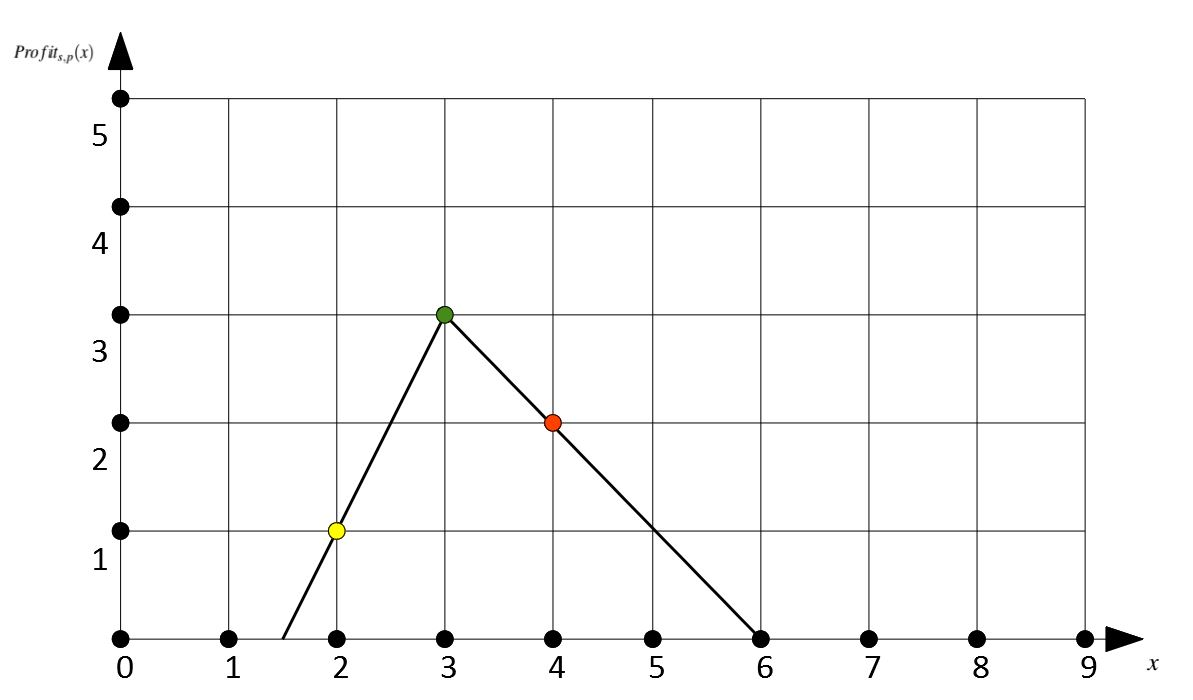
\includegraphics[scale=0.5]{profit_func}\\
\caption{A profit függvény szemléltetése}
\label{profit_func}
\end{center}
\end{figure}
Nyilvánvalóan a bevétel akkor lesz maximális, ha a kereslettel egyező darabszámot gyártunk az adott termékből (zöld pont az ábrán), ha ennél kevesebbet gyártunk a termékből, akkor a kereslet kielégítéséből eredő profit is elmarad, illetve további többlet költség kerül levonásra a profit összegéből az esetleges alul termelési plusz költségek miatt (pl. sárga pont az ábrán), abban az esetben pedig, ha a keresletet meghaladó mennyiséget gyártunk adott termékből, a kereslet kielégítődik ugyan, és bevételünk maximális lenne az adott piaci keresletet figyelembe véve, azonban a túltermelés következtében létrejött többlet tárolási költségét le kell vonjuk a profit értékéből (pl. piros pont az ábrán). Arra kell törekedni tehát, hogy a lehetőségeket mérlegelve minden termékből annyit gyártsunk, hogy az az adott forgatókönyvben szereplő keresletet kielégítse, vagy azt a legkedvezőbb módon megközelítse valamelyik irányból, ügyelve az alul-, és túltermelési költségekre. Extrém esetekben előállhat olyan helyzet is, hogy a rendelkezésre álló determinisztikus paraméterek (pl. gépek száma), az aktuális időhorizont, illetve a sztochasztikus paraméterek aktuális értéke miatt a profit függvény $x$-ben felvett értéke negatív szám lesz, ez esetben inkább a veszteségek minimalizálásáról beszélhetünk, mintsem profit maximalizálásról, azonban könnyen belátható, hogy a definiált matematikai modellekben amelyeket használunk a profit kiszámítására, ez semmiféle változást nem eredményez, csupán arra kell figyelni, hogy az implementáció során felkészüljünk a negatív számok a programnyelvben történő kezelésére.
\subsection{Preventív ütemezés fix batch mérettel}
Ebben az esetben az egyetlen döntés, amit meg kell hozni, hogy az egyes termékekből hány darab batch-et gyártsunk, a várható profit könnyen kiszámítható:
$$\sum_{p \in P}\bigg (\sum_{s \in S} prob_s \cdot profit_{s,p} (s_p \cdot b_p)\bigg)$$
Érdemes még bevezetni adott $p$ termék $x$ értékben vett várható profit értékére a következő jelölést:
$$ExpProfit_p(x)=\sum_{s \in S}prob_s \cdot profit_{s,p}(x)$$
Fontos megjegyezni, hogy az egyes termékek várható profitja egymástól független, hiszen nem osztoznak közös recepteken, éppen ezért, ha két különböző konfigurációban adott termékből gyártott batch darabszám megegyezik, akkor ha megnöveljük, vagy csökkentjük ezt a számot, mindkét konfiguráció várható profit értékében ugyan olyan változás fog történni, attól függetlenül, hogy más termékekből adott konfigurációban mennyit gyártunk.
Ezenkívül tudjuk azt is, hogy az $ExpProfit$ függvény értéke sosem fog nőni, ha már egyszer elkezdett csökkenni, mert $ExpProfit$ egy folytonos, szakaszos, lineáris függvény. \cite{?}
$ExpProfit_p(x)$ kiszámításához tehát nincs másra szükségünk, mint hogy az összes forgatókönyvre sorban felépítsünk az adott forgatókönyvre vonatkozó sztochasztikus paraméterekből a $profit_{s,p}$ függvényt, majd ezt a függvény beszorozzuk az aktuális $prob_s$ értékkel, amely lényegében a függvény "összenyomását" jelenti. Miután minden forgatókönyvre előállítottuk a \ref{profit_func_prob} ábrához hasonlóan ezt az "összenyomott" profit függvényt, ezen függvények összeadásával előáll az $ExpProfit_p$, ha ezt minden termékre megtesszük, az adott $p$ termékek $ExpProfit_p(x) \text{ (ahol }x=s_p \cdot b_p)$ értékének összegeként előáll a várható profit.
\pagebreak
\begin{figure}
\begin{center}
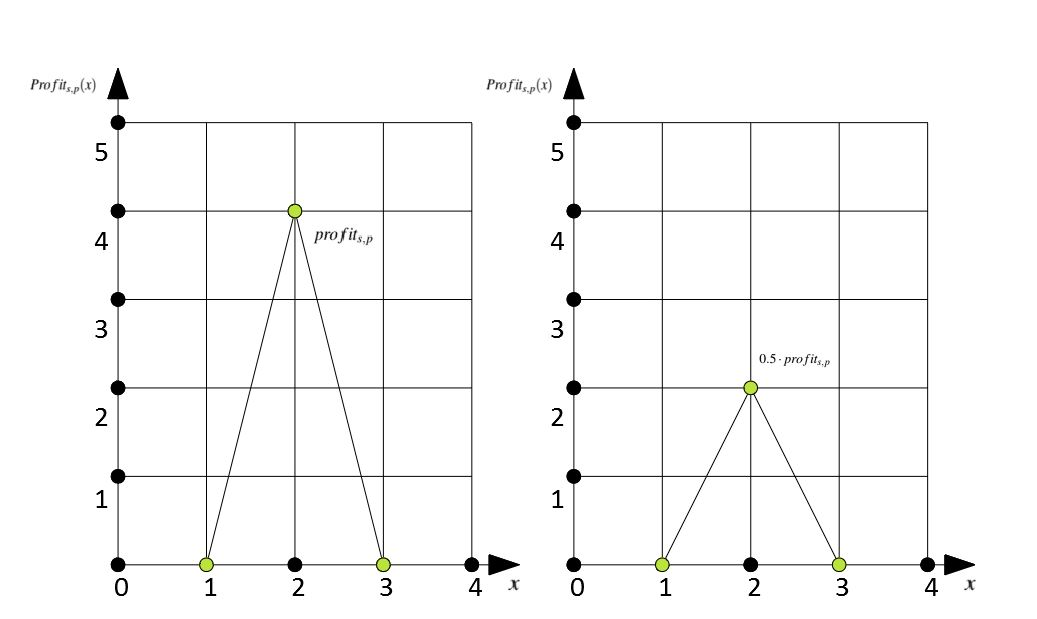
\includegraphics[scale=0.5]{profit_func_prob}
\caption{A profit függvény szorzásának szemléltetése}
\label{profit_func_prob}
\end{center}
\end{figure}
\subsection{Preventív ütemezés változó batch mérettel} \label{variable_batch_size_modell}
Az előző esettel ellentétben, változó batch méret esetén a batch darabszám nem határozza meg egyértelműen az adott termékből termelt mennyiséget. Ebben az esetben a batch méretről való döntés is a megoldó algoritmus feladata úgy, hogy $p$ termék batch mérete $s_p^{min}$ és $s_p^{max}$ között legyen. Mivel ezt a döntést előre meg kell hozni, ezért minden forgatókönyvben azonos méretű lesz minden $p$ termékhez tartozó batch. Ezután, már csak arról kell döntést hozni, hogy adott termékből mennyit gyártsunk, ez az $x_p$ érték a következő intervallumból kerül kiválasztásra: $[s_p^{min} \cdot b_p , s_p^{max} \cdot b_p]$. Az $ExpProfit$ függvény maximális értékét az egyik keresleti értékben veszi fel, legyen ez $dem_{s'}$. Az optimális $x_p$ érték kiválasztása a következőképpen tehető meg:
\begin{equation*}
x_{p}(b_p)= \begin{cases}
            b_p \cdot s_p^{max} \quad \text{ha } b_p \cdot s_p^{max}<dem_{s'}\\
            dem_{s'} \qquad \text{ha } b_p \cdot s_p^{min} \leq dem_{s'} \leq b_p \cdot s_p^{max}\\
            b_p \cdot s_p^{min} \quad \text{ ha } b_p \cdot s_p^{min}>dem_{s'}
       \end{cases}       
\end{equation*}\\
A \ref{expProfit_func_var} ábra szemlélteti a fentieket. Látható, hogy ez esetben a $dem_{s'}$ érték beleesik a \\$[s_p^{min} \cdot b_p , s_p^{max} \cdot b_p]$ tartományba, ezért itt $x_p=3$ lenne az optimális választás.
\begin{figure}
\begin{center}
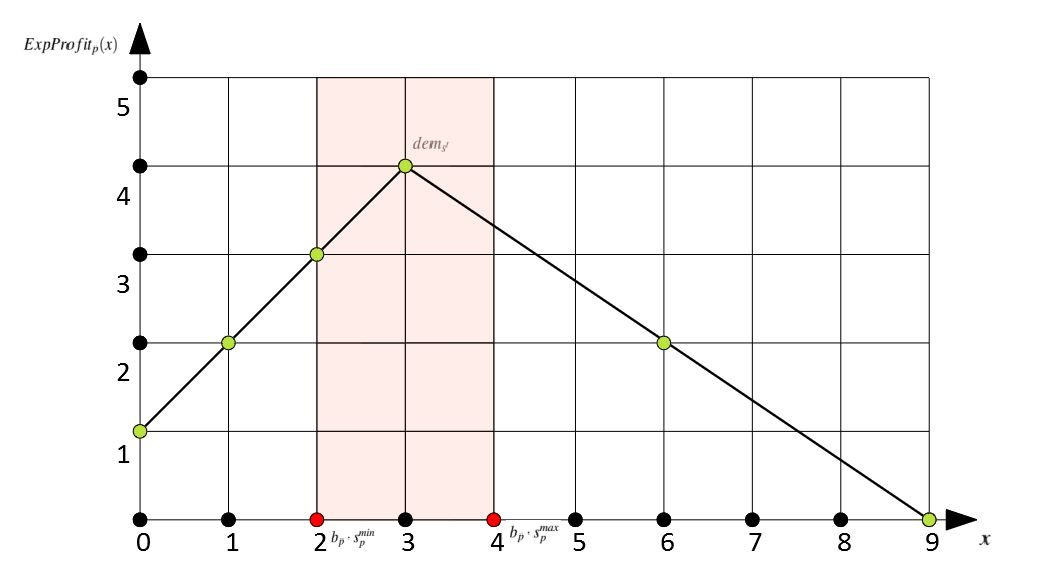
\includegraphics[scale=0.5]{expProfit_func_var}
\caption{Az optimális $x_p$ érték kiválasztásának szemléltetése}
\label{expProfit_func_var}
\end{center}
\end{figure}
\subsection{Two stage (két lépcsős ütemezés)}
Ebben az esetben $p$ termék gyártandó mennyiségét illető döntés egy bizonytalan esemény bekövetkezése után is meghozható, például, ha egy forgatókönyv már bekövetkezett. Éppen ezért a termék mennyisége az adott forgatókönyvtől függ, legyen ez: $x_{s,p}$. E mennyiség kiválasztása a következőképpen zajlik:
\begin{equation*}
x_{s,p}(b_p)= \begin{cases}
            b_p \cdot s_p^{max} \quad \text{ha } b_p \cdot s_p^{max}<dem_{s}\\
            dem_{s} \qquad \text{ha } b_p \cdot s_p^{min} \leq dem_{s} \leq b_p \cdot s_p^{max}\\
            b_p \cdot s_p^{min} \quad \text{ ha } b_p \cdot s_p^{min}>dem_{s}
       \end{cases}       
\end{equation*}\\
Látható, hogy a képlet hasonló a \ref{variable_batch_size_modell} pontban bemutatott képlethez, azonban míg ott  az $ExpProfit$ függvényből kerül kiválasztásra az optimális $x_p$ mennyiség (azaz, minden forgatókönyv esetén ez az érték ugyan annyi lesz), addig a két lépcsős ütemezés esetén minden egyes forgatókönyv $Profit$ függvényéből egyenként kerül kiválasztásra az optimális mennyiség. Ezzel megoldható az, hogy egy bizonyos forgatókönyv bekövetkezése után annak elvárásaihoz igazítsuk a termelt batch-ek méretét, jobb várható profitot elérve ezzel a legtöbb esetben. A várható profit két lépcsős ütemezés esetén a következőképpen számítható ki:
$$\sum_{p \in P} \bigg( \sum_{s \in S}(prob_s \cdot Profit(x_{s,p}(b_p)) \bigg)$$ 
\subsection{Következtetés} \label{broken_line_suggestion}
A matematikai modellek ismerete arra enged következtetni, hogy a probléma az \ref{s-graph_framework}. fejezetben bemutatott S-gráf keretrendszerbe történő integrálásához elengedhetetlen lesz egy olyan osztály definiálása, amely képes  folytonos, szakaszos, lineáris függvények modellezésére, tárolására, azokon történő műveletek végrehajtására. Ezen osztály részletes leírása a \ref{broken_line_class} pontban olvasható.
\chapter{Az S-gráf keretrendszer} \label{s-graph_framework}
\chapter{A probléma megvalósítása}
\section{A BrokenLine osztály} \label{broken_line_class}
Ahogy az már korábban, a \ref{broken_line_suggestion} pontban említésre került, a probléma implementációjához elengedhetetlen egy olyan osztály definiálása, amely kezelni képes folytonos, szakaszos, lineáris függvényeket. Erre hivatott az általam megalkotott \textit{BrokenLine} osztály, amelynek forráskódja \textit{brokenline.h}, illetve \textit{brokenline.cpp} fájlokban található a solver \textit{src\textbackslash base} mappájában. Az általunk használt függvények tárolásához elegendő, ha kezdetben három pont koordinátái adottak, hiszen ezek elhelyezkedéséből a többi pont koordinátái később, ha valamilyen okból kifolyólag ez szükségessé válik, könnyen kiszámíthatóak, hiszen folytonos, lineáris függvényekről beszélünk. Ez a három pont a $profit_{s,p}$ függvények esetében nem más, mint: 
\begin{itemize}
\item $Profit_{s,p}(x)$\quad, ahol $x=dem_{s,p}-1$
\item $Profit_{s,p}(x)$\quad, ahol $x=dem_{s,p}$
\item $Profit_{s,p}(x)$\quad, ahol $x=dem_{s,p}+1$
\end{itemize} 
E három pont koordinátái minden esetben kiszámíthatók, minden forgatókönyv-termék párosra már az input fájl beolvasását követően, hiszen minden sztochasztikus paraméter adott ehhez a fájlban. Az ehhez szükséges képlet a \ref{variable_batch_size_modell} pont szerint:
\begin{equation*}
Profit_{s,p}(x)= \begin{cases}
            price_{s,p}\cdot x-(dem_{s,p}-x) \cdot uc_{s,p}\qquad \text{ha } x<dem_{s,p} \\
            price_{s,p} \cdot dem_{s,p}-(x-dem_{s,p}) \cdot oc_{s,p}\qquad \text{egyébként}
       \end{cases}
\end{equation*}
Miután ennek a három pontnak a pontos koordinátái beazonosításra kerültek, már csak annyit kell tenni, hogy kiszámítunk két arány számot, amelyek a függvény kezdeti-, és vég meredekségét hivatottak letárolni. Ezen paraméterek ismeretében később a függvény bármely $x$ pontjában felvett értéke számítható lesz. Ezek alapján a \textit{BrokenLine} osztály adattagjai a következőek:
\begin{figure}[H]
\begin{center}
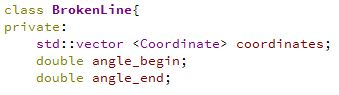
\includegraphics[scale=1]{broken_line_variables}
\caption{A \textit{BrokenLine} osztály adattagjai}
\label{broken_line_variables}
\end{center}
\end{figure} 
A \ref{broken_line_variables} ábrán látható \textit{Coordinate} osztály a függvények pontjainak $x$ és $y$ koordinátáinak egyszerű tárolására, lekérdezésére, és összehasonlítására szolgál a megvalósított \textit{setter}, \textit{getter} és felültöltött egyenlőség operátorral.\\
Ahhoz, hogy a \textit{BrokenLine} osztállyal a matematikai modellek minden szükséges művelete elvégezhető legyen, a következő funkcionalitást kell megvalósítani az osztálynak:
\begin{itemize}
\item Koordináta pár hozzáadása
\item Koordináta párok rendezése $x$ szerint növekvő sorrendbe
\item Kezdeti-, és vég meredekség kiszámítása
\item A függvény skalár értékkel való szorzása
\item A függvény $x$ helyen vett értékének lekérdezése
\item Két függvény összeadása
\item A függvény horizontális nyújtása (a \ref{extended_multiproduct} pontban tárgyalt esetekhez)
\item A függvény maximális értékéhez tartozó koordináták lekérdezése
\end{itemize} 
\subsection{Koordináta pár hozzáadása} \label{addCoordinates}
Egy új koordináta pár hozzáadását végző metódus az \textit{addCoordinate(const Coordinate\& c)}. Egy új koordináta pár hozzáadása esetén először is meg kell győződnünk, hogy adott koordináta pár szerepel-e már a koordináták tárolására szolgáló vectorban, hiszen ha már szerepel, nem adhatjuk hozzá újra. Ha nem szerepel még ilyen koordináta pár, hozzáadjuk, majd rendezzük a vectort $x$ szerint növekvő sorrendbe. Ha ez megtörtént, meg kell vizsgálni, hogy a kezdeti-, és vég meredekségeket frissíteni kell-e. Abban az esetben, ha a most hozzáadott koordináta pár szerepel a rendezett vector első, vagy második helyén, a kezdeti meredekséget frissíteni kell. Hasonlóan, ha az új koordináta pár a vector utolsó, vagy utolsó előtti eleme, a vég meredekség frissítésre szorul. Mivel kezdetben akár mindkét feltétel igaz lehet, ezért ezek teljesülését két külön \textit{bool} változóban kell tárolni. Miután megállapításra került, hogy melyik meredekségeket kell frissíteni, meghívásra kerül az ezeket kiszámító függvény. 
\subsection{Kezdeti-, és vég meredekség kiszámítása} \label{calculateAngle}
A  kezdeti-, és vég meredekség kiszámítására és frissítésére hivatott metódus a \textit{calculateAngle(bool begin,bool end)}, melynek két paramétere a \ref{addCoordinates} pontban említett két \textit{bool} változó, amelyek megadják, hogy kell e frissíteni adott meredekségeket. A meredekségek kiszámítása roppant egyszerű a koordináták ismeretében:
$$Angle_{begin}=(y_{second}-y_{first}) / (x_{second}-x_{first})$$
$$Angle_{end}=(y_{penultimate}-y_{last}) / (x_{last}-x_{penultimate})$$
A \ref{calculate angle} ábrán látható három pont koordinátái alapján a meredekségek például a következőképpen alakulnak: 
$$Angle_{begin}=(4-3) / (3-2)\quad \text{, azaz } Angle_{begin}=1$$
$$Angle_{end}=(4-2) / (6-3)\quad \text{, azaz } Angle_{end}=2/3$$
\begin{figure}[H]
\begin{center}
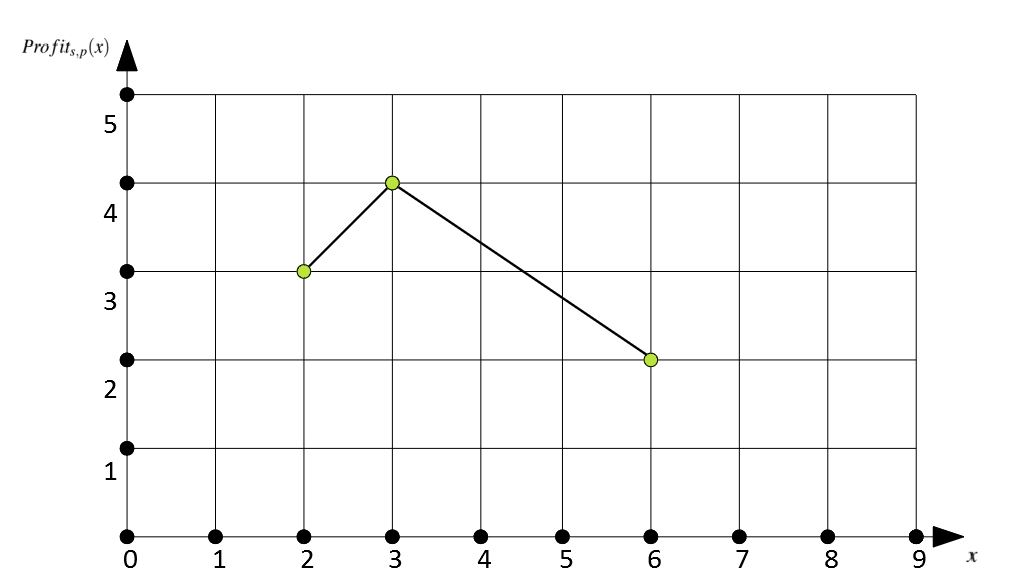
\includegraphics[scale=0.5]{calculate_angle}
\caption{Példa a meredekségek kiszámítására}
\label{calculate angle}
\end{center}
\end{figure}
Ha egyik meredekség sem szorul frissítésre, a metódus semmiféle változtatást nem tesz.
\subsection{A függvény skalár értékkel való szorzása} \label{multiplyByScalar}
A függvény skalárral való szorzását a \textit{multiplyByScalar(double s)} metódus végzi. Ahhoz, hogy megkapjuk a függvény skalárral való szorzatát, csupán be kell szorozni a vectorban tárolt összes pont $y$ koordinátáját, valamint a kezdeti-, és vég meredekséget a paraméterként kapott $s$-el. A függvény szorzását szemléltető példa a \ref{profit_func_prob} ábrán látható.
\subsection{A függvény $x$ helyen vett értékének lekérdezése} \label{getValue}
A függvény $x$ helyen vett értékének lekérdezésére a \textit{getValue(double x)} metódus hivatott. A metódus először is megnézi, hogy a vectorban tárolt koordináta párok között található-e olyan, amelynek $x$ koordinátája egyezik a paraméterként kapott $x$-el. Ha talál ilyet, egyszerűen visszaadja a megfelelő koordináta párost tartalmazó \textit{Coordinate} objektumot. Ha nem található ilyen pont, akkor annak ki kell számítani a koordinátáit, és hozzá kell adni a vectorhoz, majd csak azután lehet visszaadni a keresett \textit{Coordinate} objektumot. Az $x$ értékhez tartozó $y$ érték kiszámítása a keresett $x$ értéke és a vectorban tárolt pontok alapján háromféleképpen történhet:
\begin{itemize}
\item Ha a keresett $x$ értéke kisebb mint a vectorban tárolt első pont $x$ koordinátájának értéke, akkor: 
$y=y_{First}-(x_{First}-x) \cdot Angle_{begin}$ ,ahol $x_{First} \text{ és } y_{First}$ a vectorban tárolt első pont koordinátái.
\item Ha a keresett $x$ érték két a vectorban tárolt pont $x$ koordinátájának értéke közé esik, akkor:
$y=\bigg(\big(x-x_{LastSmaller}\big) \cdot \big((y_{FirstBigger}-y_{LastSmaller})/(x_{FirstBigger}-x_{LastSmaller})\big)\bigg)+y_{LastSmaller}$
\end{itemize}
\subsection{Két függvény összeadása} \label{addBrokenLine}
Két függvény összeadását az \textit{addBrokenLine(BrokenLine b)} metódus végzi, melynek visszatérési értéke az összegként kapott függvényt tároló új \textit{BrokenLine} objektum. Mivel a függvények tárolásához elegendő három pont tárolása, ezért gyakran előfordul olyan eset, hogy a két összeadni kívánt \textit{BrokenLine} objektum nem tartalmazza a szükséges koordinátákat, ezért a hiányzó koordináta párokat először hozzá kell adni   
\section{Szükséges változtatások az általános throughput maximalizálón} \label{refactor}
\section{Multiproduct receptek esete} \label{extended_multiproduct}
\chapter{Teszteredmények}
\chapter{Összefoglalás}

\end{document}